In order to evaluate and validate the approach proposed in this paper, we have
conducted experiments on simulated and real-world data. We shall first start
with the description of the experimental conditions and then demonstrate the
performance of our algorithm, along with some comparisons against existing
methods.

\subsection{Experimental Setup}

Our method has been fully implemented in MATLAB and we have used the
SuiteSparseQR~\cite{davis11algorithm} package for performing sparse matrices
operations.

Although our eventual goal is full, self-supervised calibration for an
autonomous vehicle system with multiple heterogeneous sensors, the
experiments in this paper are based on a realistic, but somewhat
simplified robotic system. This allows us to precisely control the
observability properties in simulation and test the behavior of our
algorithm.

Fig.~\ref{fig:exp_setup} depicts our experimental setup. The platform
is a differential drive mobile robot equipped with a range sensor
delivering range and bearing measurements. The calibration parameters
of the range sensor consist in the transformation of its coordinate
system to the robot's coordinate system. The platform is further
endowed with wheel odometers outputting translational and rotational
speeds. While navigating on the plane, the robot observes a known
number of landmarks through its range sensor. Both the range sensor 
and the odometry produce data at 10 Hz.

\begin{figure}[t]
\centering
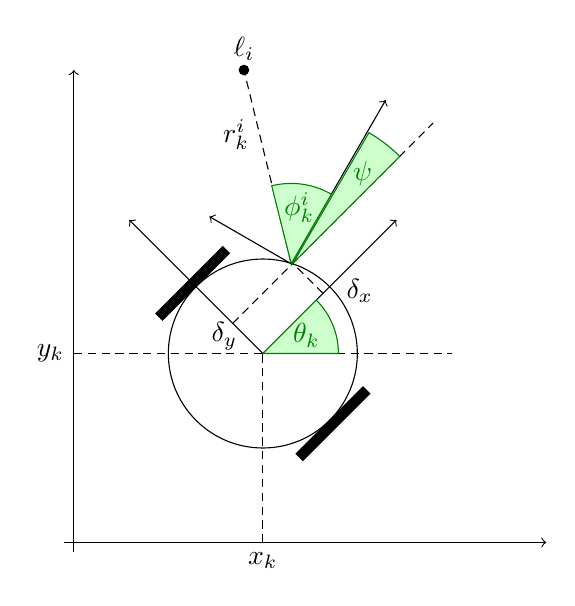
\begin{tikzpicture}[scale = 1.2]
  % styles
\tikzstyle{axes}=[]
\tikzstyle{robot} = []
\tikzstyle{wheels} = [fill]
\tikzstyle{landmark} = [fill]
\tikzstyle{lrf measurement} = [densely dashed]
\colorlet{anglecolor}{green!50!black}

% world axes
\begin{scope}[style = axes]
  \draw[->] (-0.1, 0) -- (5, 0);
  \draw[->] (0, -0.1) -- (0, 5);
\end{scope}

% robot base
\begin{scope}[style = robot, xshift = 2cm, yshift = 2cm, rotate = 45]
  \draw (0, 0) circle (1);
  \draw[wheels] (-0.5, 1) rectangle (0.5, 1.1);
  \draw[wheels] (-0.5, -1) rectangle (0.5, -1.1);
\end{scope}

% robot axes
\begin{scope}[style = axes, xshift = 2cm, yshift = 2cm, rotate = 45]
  \draw[->] (0, 0) -- (2, 0);
  \draw[->] (0, 0) -- (0, 2);
\end{scope}

% lrf axes
\begin{scope}[style = axes, xshift = 2.3cm, yshift = 2.95cm, rotate = 60]
  \draw[->] (0, 0) -- (2, 0);
  \draw[->] (0, 0) -- (0, 1);
\end{scope}

% landmark
\begin{scope}[style = landmark, xshift = 1.8cm, yshift = 5cm, rotate = 0]
  \draw[landmark] (0, 0) circle (0.05) node[above] {$\boldsymbol{\ell}_i$};
\end{scope}

% lrf range measurement
\begin{scope}[style = lrf measurement]
  \draw (2.3, 2.95) -- (1.8, 5) node[left = 0.1cm, below = 0.5cm] {$r^i_k$};
\end{scope}

% lrf bearing measurement
\begin{scope}[xshift = 2.3cm, yshift = 2.95cm, rotate = 60]
  \filldraw[fill = green!20, draw = anglecolor] (0, 0) -- (8.5mm, 0) arc
    (0:44:8.5mm) -- cycle;
  \draw (22:6mm) node[anglecolor] {$\phi^i_k$};
\end{scope}

% robot pose
\begin{scope}
  \draw[densely dashed] (2, 0) node[below] {$x_k$} -- (2, 2);
  \draw[densely dashed] (0, 2) node[left] {$y_k$} -- (4, 2);
  \filldraw[fill = green!20, draw = anglecolor] (2, 2) -- (2.8, 2) arc
    (0:45:0.8) -- cycle;
  \draw[xshift = 2cm, yshift = 2cm] (22.5:0.5) node[anglecolor] {$\theta_k$};
\end{scope}

% lrf pose
\begin{scope} [xshift = 2cm, yshift = 2cm, rotate = 45]
  \draw[densely dashed] (0.9, 0) node[below = -1pt, right = 5pt] {$\delta_x$}
    -- (0.9, 0.45);
  \draw[densely dashed] (0, 0.45) node[left = 3pt, below = -3.8pt] {$\delta_y$}
    -- (3, 0.45);
  \filldraw[fill = green!20, draw = anglecolor] (0.9, 0.45) -- (2.5, 0.45) arc
    (0:14.8:1.6) -- cycle;
  \draw[xshift = 0.9cm, yshift = 0.45cm] (7:1.2) node[anglecolor] {$\psi$};
\end{scope}

\end{tikzpicture}
\caption{Experimental setup. A 2D robot moving in a plane and observing
  landmarks with a range sensor providing range and bearing angle measurements.
  The calibration process needs to find the 2D transformation between the
  robot's coordinate system and the sensor's coordinate system.}
\label{fig:exp_setup}
\end{figure}

More formally, we adopt the following motion and observation models

\begin{equation}\label{eqn:exp_model}
  \begin{aligned}
  \underbrace {
  \begin{pmatrix}
  x_k\\
  y_k\\
  \theta_k
  \end{pmatrix}}_{\mathbf{x}_k}&=
  \underbrace{
  \begin{pmatrix}
  x_{k-1}\\
  y_{k-1}\\
  \theta_{k-1}
  \end{pmatrix} + T
  \begin{pmatrix}
  \cos\theta_{k-1}&0\\
  \sin\theta_{k-1}&0\\
  0&1
  \end{pmatrix}
  \left(\begin{pmatrix}
  v_k\\
  w_k
  \end{pmatrix}
  + \mathbf{w}_k\right)
  }_{\mathbf{h}(\mathbf{x}_{k-1}, \mathbf{u}_k, \mathbf{w}_k)}\\
  a &= x_i - x_k - \delta_x\cos\theta_k + \delta_y\sin\theta_k\\
  b &= y_i - y_k - \delta_x\sin\theta_k - \delta_y\cos\theta_k\\
  \underbrace {
  \begin{pmatrix}
  r_k^i\\
  \phi_k^i
  \end{pmatrix} }_{\mathbf{z}_{k_i}}&=
  \underbrace {
  \begin{pmatrix}
  \sqrt{a^2 + b^2}\\
  \atan2(b, a) - \theta_k - \psi
  \end{pmatrix}
  + \mathbf{n}_k}_{\mathbf{g}(\mathbf{x}_{k}, \boldsymbol{\ell}_i,
    \boldsymbol{\Theta}, \mathbf{n}_k)},
  \end{aligned}
\end{equation}

\noindent where $\mathbf{x}_k=[x_k\;y_k\;\theta_k]^T$ denotes the robot pose at
timestep $k$, $T$ the sampling period, $\mathbf{u}_k=[v_k\;w_k]^T$ the measured
translational and rotational speeds, $\mathbf{z}_{k_i}=[r_k^i\;\phi_k^i]^T$ the
range and bearing observation of landmark $i$ with pose
$\boldsymbol{\ell}_i=[x_i\;y_i]^T$, $\mathbf{w}_k\sim\mathcal{N}(\mathbf{0},
\mathbf{W}_k)$ with $\mathbf{W}_k=\diag(\sigma^2_v,\sigma^2_w)$,
$\mathbf{n}_k\sim\mathcal{N}(\mathbf{0}, \mathbf{N}_k)$ with
$\mathbf{N}_k=\diag(\sigma^2_r,\sigma^2_\phi)$, and
$\mathbf{\Theta}=[\delta_x\;\delta_y\;\psi]^T$ the range sensor's calibration
parameters.

Throughout our experiments, we have used a non-informative prior
$p(\boldsymbol{\Theta}, \mathbf{x}_0, \mathcal{L})$, i.e., a uniform
distribution. The use of priors is still subject to controversial
discussions~\cite{gelman08objections} between Bayesian and non-Bayesian
statisticians. Here, we argue that everything should come from the data itself
and not from some subjective prior information that could bias the inference.

Our algorithm requires only 3 free parameters, namely the rank threshold
$\epsilon$, the batch size $k$, and the MI threshold $\lambda$. Optimally, $k$
should be inferred from the dynamics of the system. While a large $k$
induces storage of uninformative measurements, a small $k$ leads to useless
runs of optimization and makes it difficult to discover informative sequences 
of measurements. In this
setup, we have used a batch size of $k=100$ (ten seconds of data). Concerning
the MI threshold, a small $\lambda$ will keep most of the measurements and a
large $\lambda$ will ignore them all. We have set this value to
$\lambda=0.5$ [bits] in our experiments. The $\epsilon$ parameter shall be
discussed below.

\subsection{Simulated Data}

In our simulation environment, we can generate various paths for the robot,
along with corresponding sensor measurements, and thus analyze the behavior of
multiple algorithms, especially in degenerate cases. We have created an
environment with $N=17$ landmarks uniformly distributed on a $20m\times 20m$
grid. We have set the noise parameters empirically to
$\sigma^2_v=4.4\times 10^{-3}$, $\sigma^2_w=8.2\times 10^{-2}$,
$\sigma^2_r=9.0036\times 10^{-4}$, and $\sigma^2_\phi=6.7143\times 10^{-4}$. The
calibration parameters are fixed at $\delta_x=0.219$ [m], $\delta_y=0.1$ [m],
and $\psi=\pi/4$ [rad].

In a first effort, we want to support the claims of Sec.~\ref{sec:tsvd} with
a representative example. We simulated the robot driving along a straight
path as shown in Fig.~\ref{fig:straight-path}. Intuitively, the problem is
structurally unobservable. Indeed, it has 5 unobservable parameters, 3
corresponding to the global pose of the map and trajectory (as no global
measurements or prior are included) and 2 for the calibration offset variables
$\delta_x$ and $\delta_y$. If we set the noise matrices $\mathbf{W}_k$ and
$\mathbf{N}_k$ to $\mathbf{0}$ and examine the singular values of the Jacobian
matrix, 5 values are $0$ up to machine precision, i.e., a structural rank
deficiency. By adding noise to the system, only 3 singular values remain at $0$
for the same problem. From the integrated odometry path in
Fig.~\ref{fig:straight-path}, the calibration parameters appear indeed as
observable and a naive algorithm without regularization will thus wrongly
optimize. Fig.~\ref{fig:straight-path-analysis} shows the singular values in
these two cases and the related concept in the QR decomposition. With our
TSVD/TQR method, we can deal with this issue by setting an adequate $\epsilon$
threshold that will recover the correct rank deficiency and therefore only
optimize the observable parts. The threshold is application-specific and should
be a function of the system noise. Obviously, at a certain level of noise, gaps
in the singular values spectrum become indistinguishable. In our setup, we have
determined the threshold empirically from the scaled system
\eqref{eqn:scaled_system} and set it to $\epsilon=0.013$.

\begin{figure}[t]
\centering
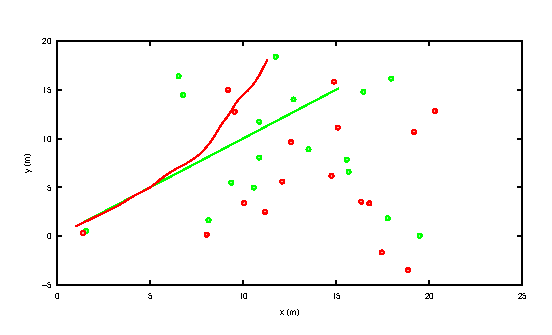
\includegraphics[width=\columnwidth]{fig/straight-path.eps}
\caption{Straight path example (best viewed in color). The green line
  represents the ground truth path, the red line the integrated odometry path,
  the green crosses the ground truth landmark positions, and the red crosses the
  guessed landmark positions from measurements.}
\label{fig:straight-path}
\end{figure}

\begin{figure}[t]
\centering
\begin{minipage}{.492\columnwidth}
  \centering
  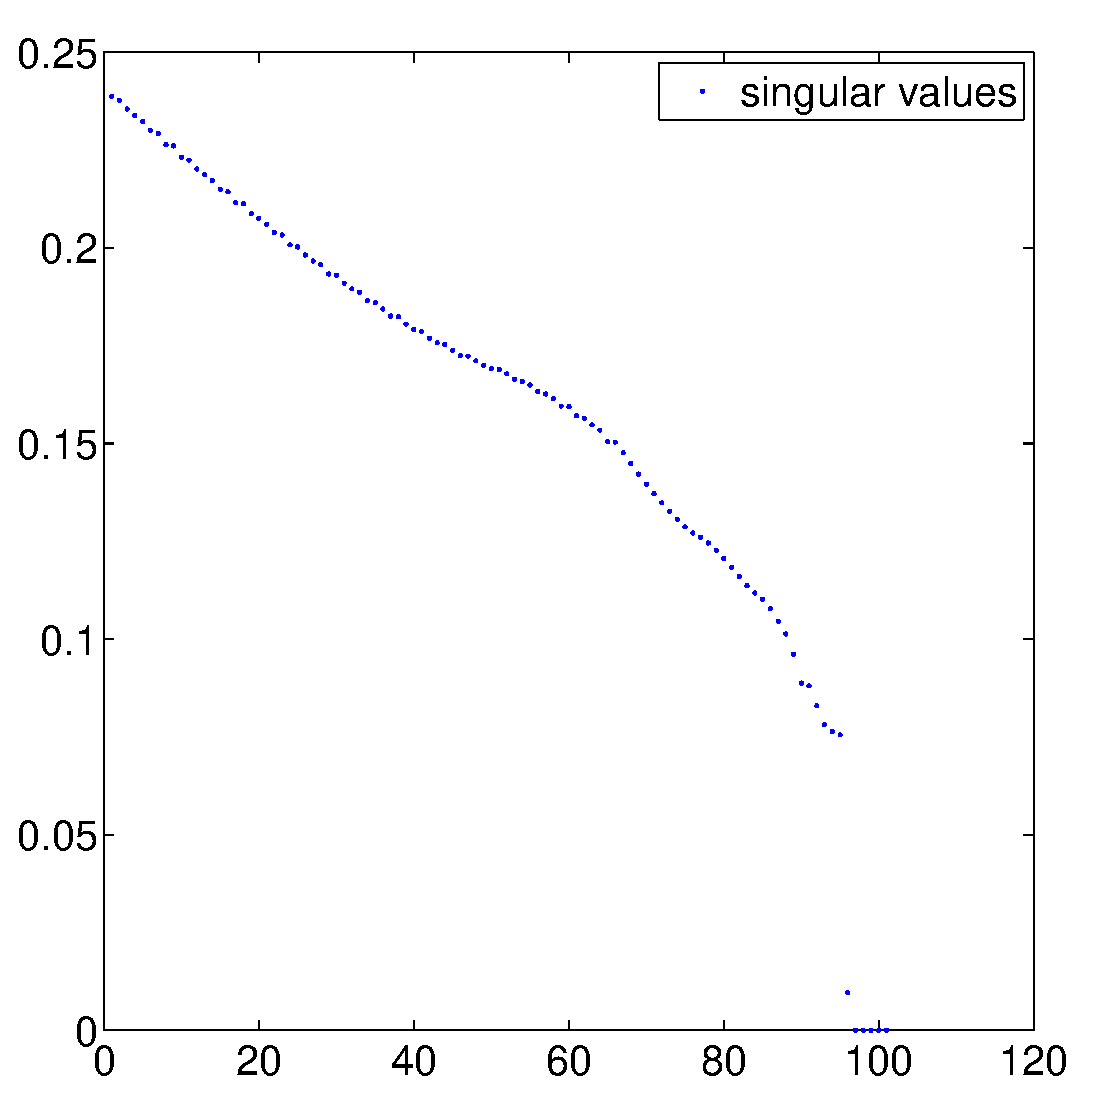
\includegraphics[width=\columnwidth]
    {fig/straight-path-noisefree-svd-scaled.eps}
\end{minipage}
\begin{minipage}{.492\columnwidth}
  \centering
  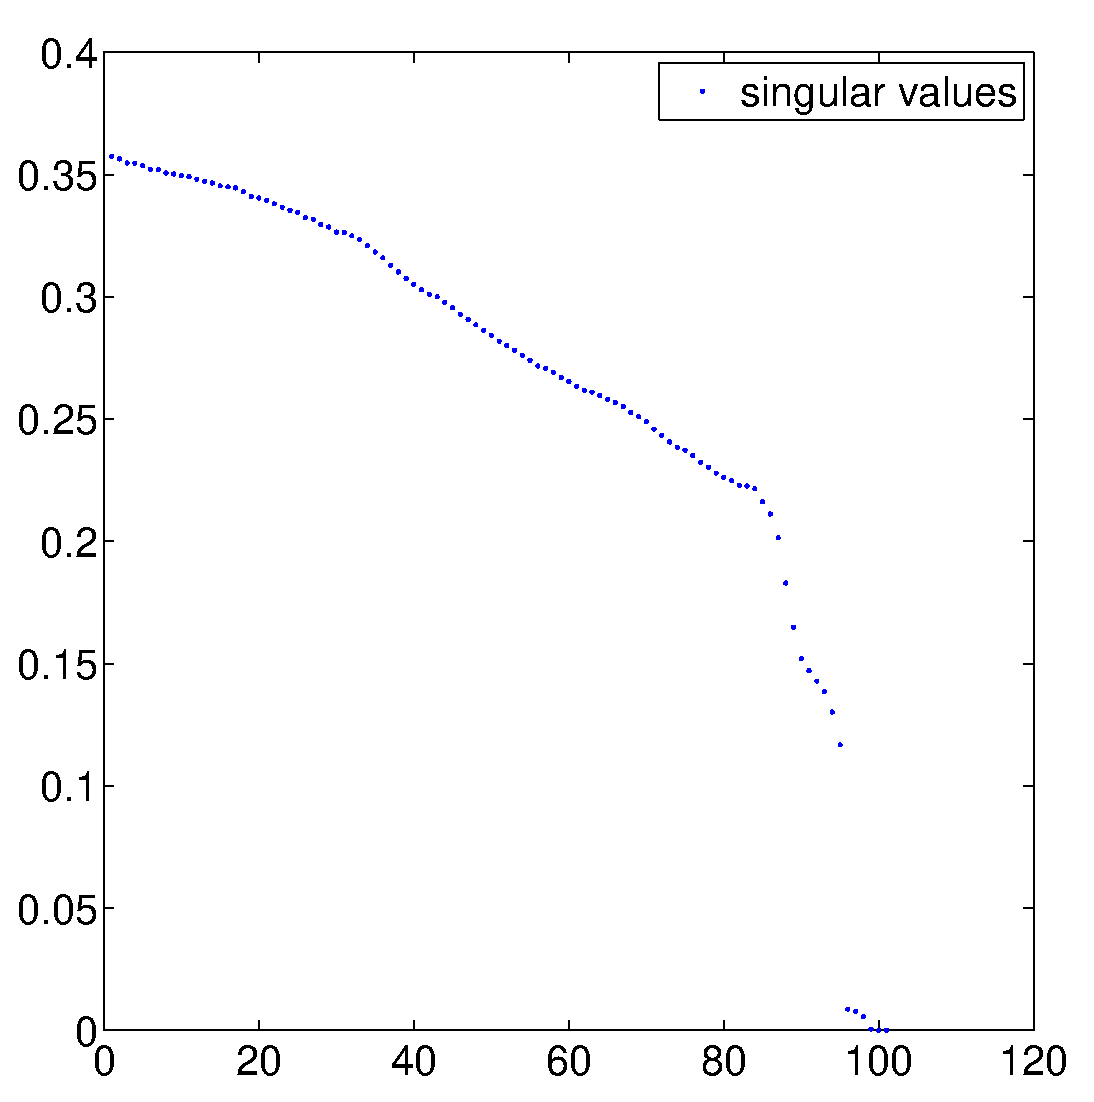
\includegraphics[width=\columnwidth]
    {fig/straight-path-svd-scaled.eps}
\end{minipage}
\begin{minipage}{.492\columnwidth}
  \centering
  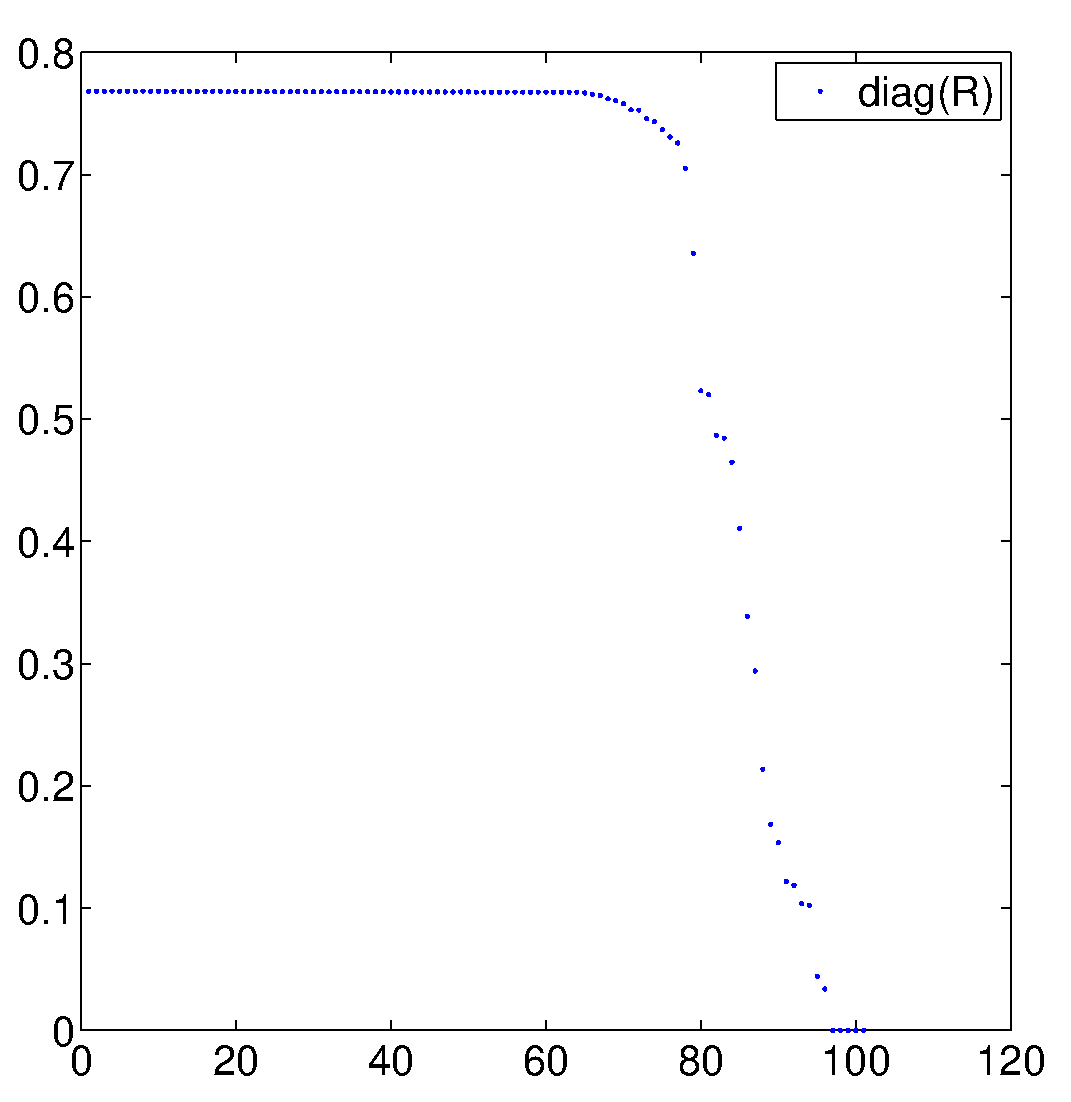
\includegraphics[width=\columnwidth]
    {fig/straight-path-noisefree-spqr-scaled.eps}
\end{minipage}
\begin{minipage}{.492\columnwidth}
  \centering
  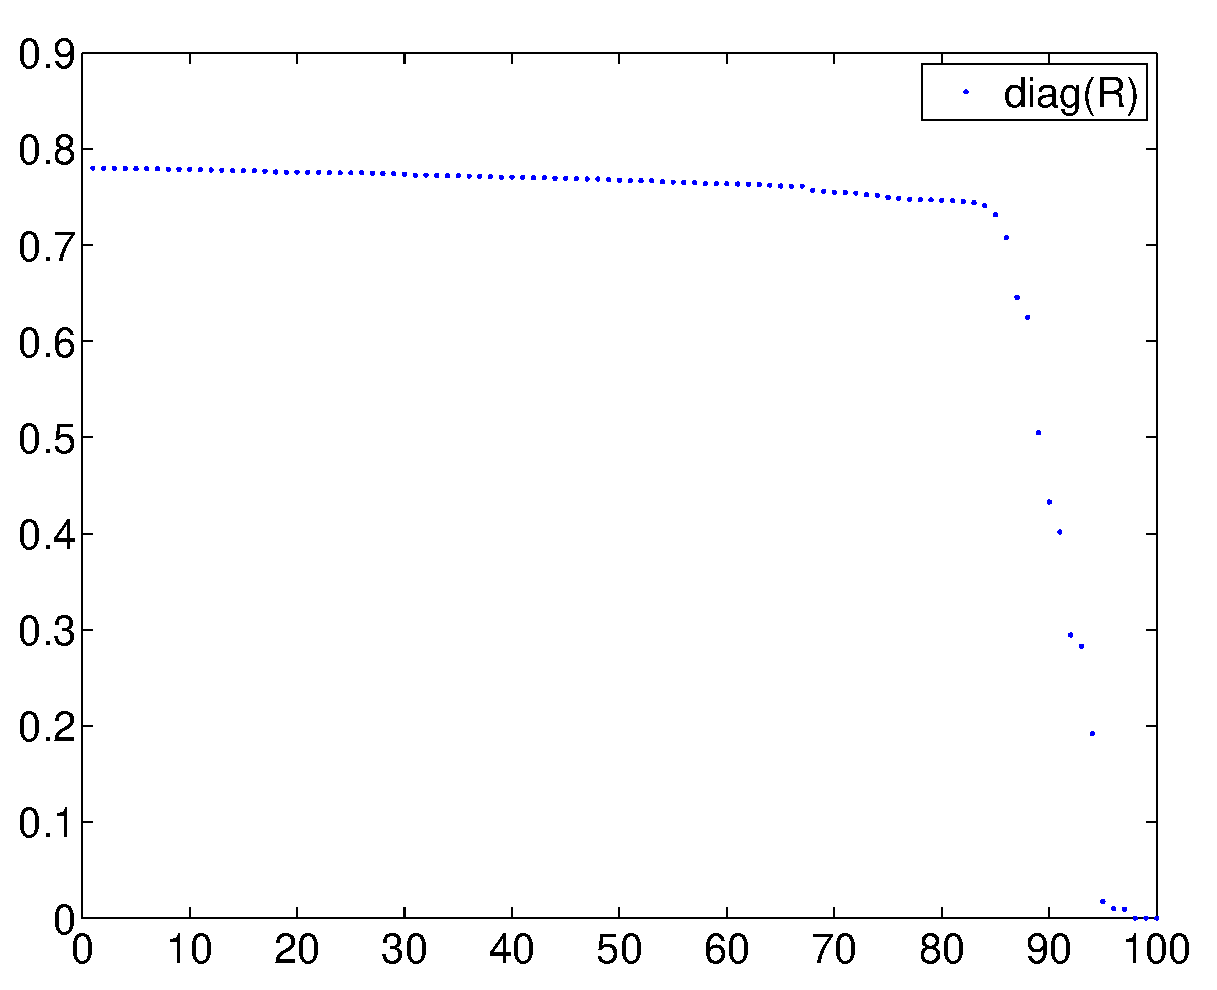
\includegraphics[width=\columnwidth]
    {fig/straight-path-spqr-scaled.eps}
\end{minipage}
\caption{Straight path example analysis. The first column shows the singular
  values and the diagonal elements of the $\mathbf{R}$ matrix from the QR
  decomposition in the noise-free case, and the second column in the noisy
  case. Only the 100 lower values from the scaled system
  \eqref{eqn:scaled_system} are plotted for visualization purpose.}
\label{fig:straight-path-analysis}
\end{figure}

For this first example, Fig.~\ref{fig:straight-path-time} shows the mean
computation time for some dataset sizes over 100 repetitions for one iteration
of the Gauss-Newton algorithm using SVD and sparse QR decomposition on a
quad-core desktop machine. It usually takes less than 10 iterations for the
optimization to converge. Nevertheless, the SVD method rapidly becomes
prohibitive due to the polynomial computation time.

\begin{figure}[t]
\centering
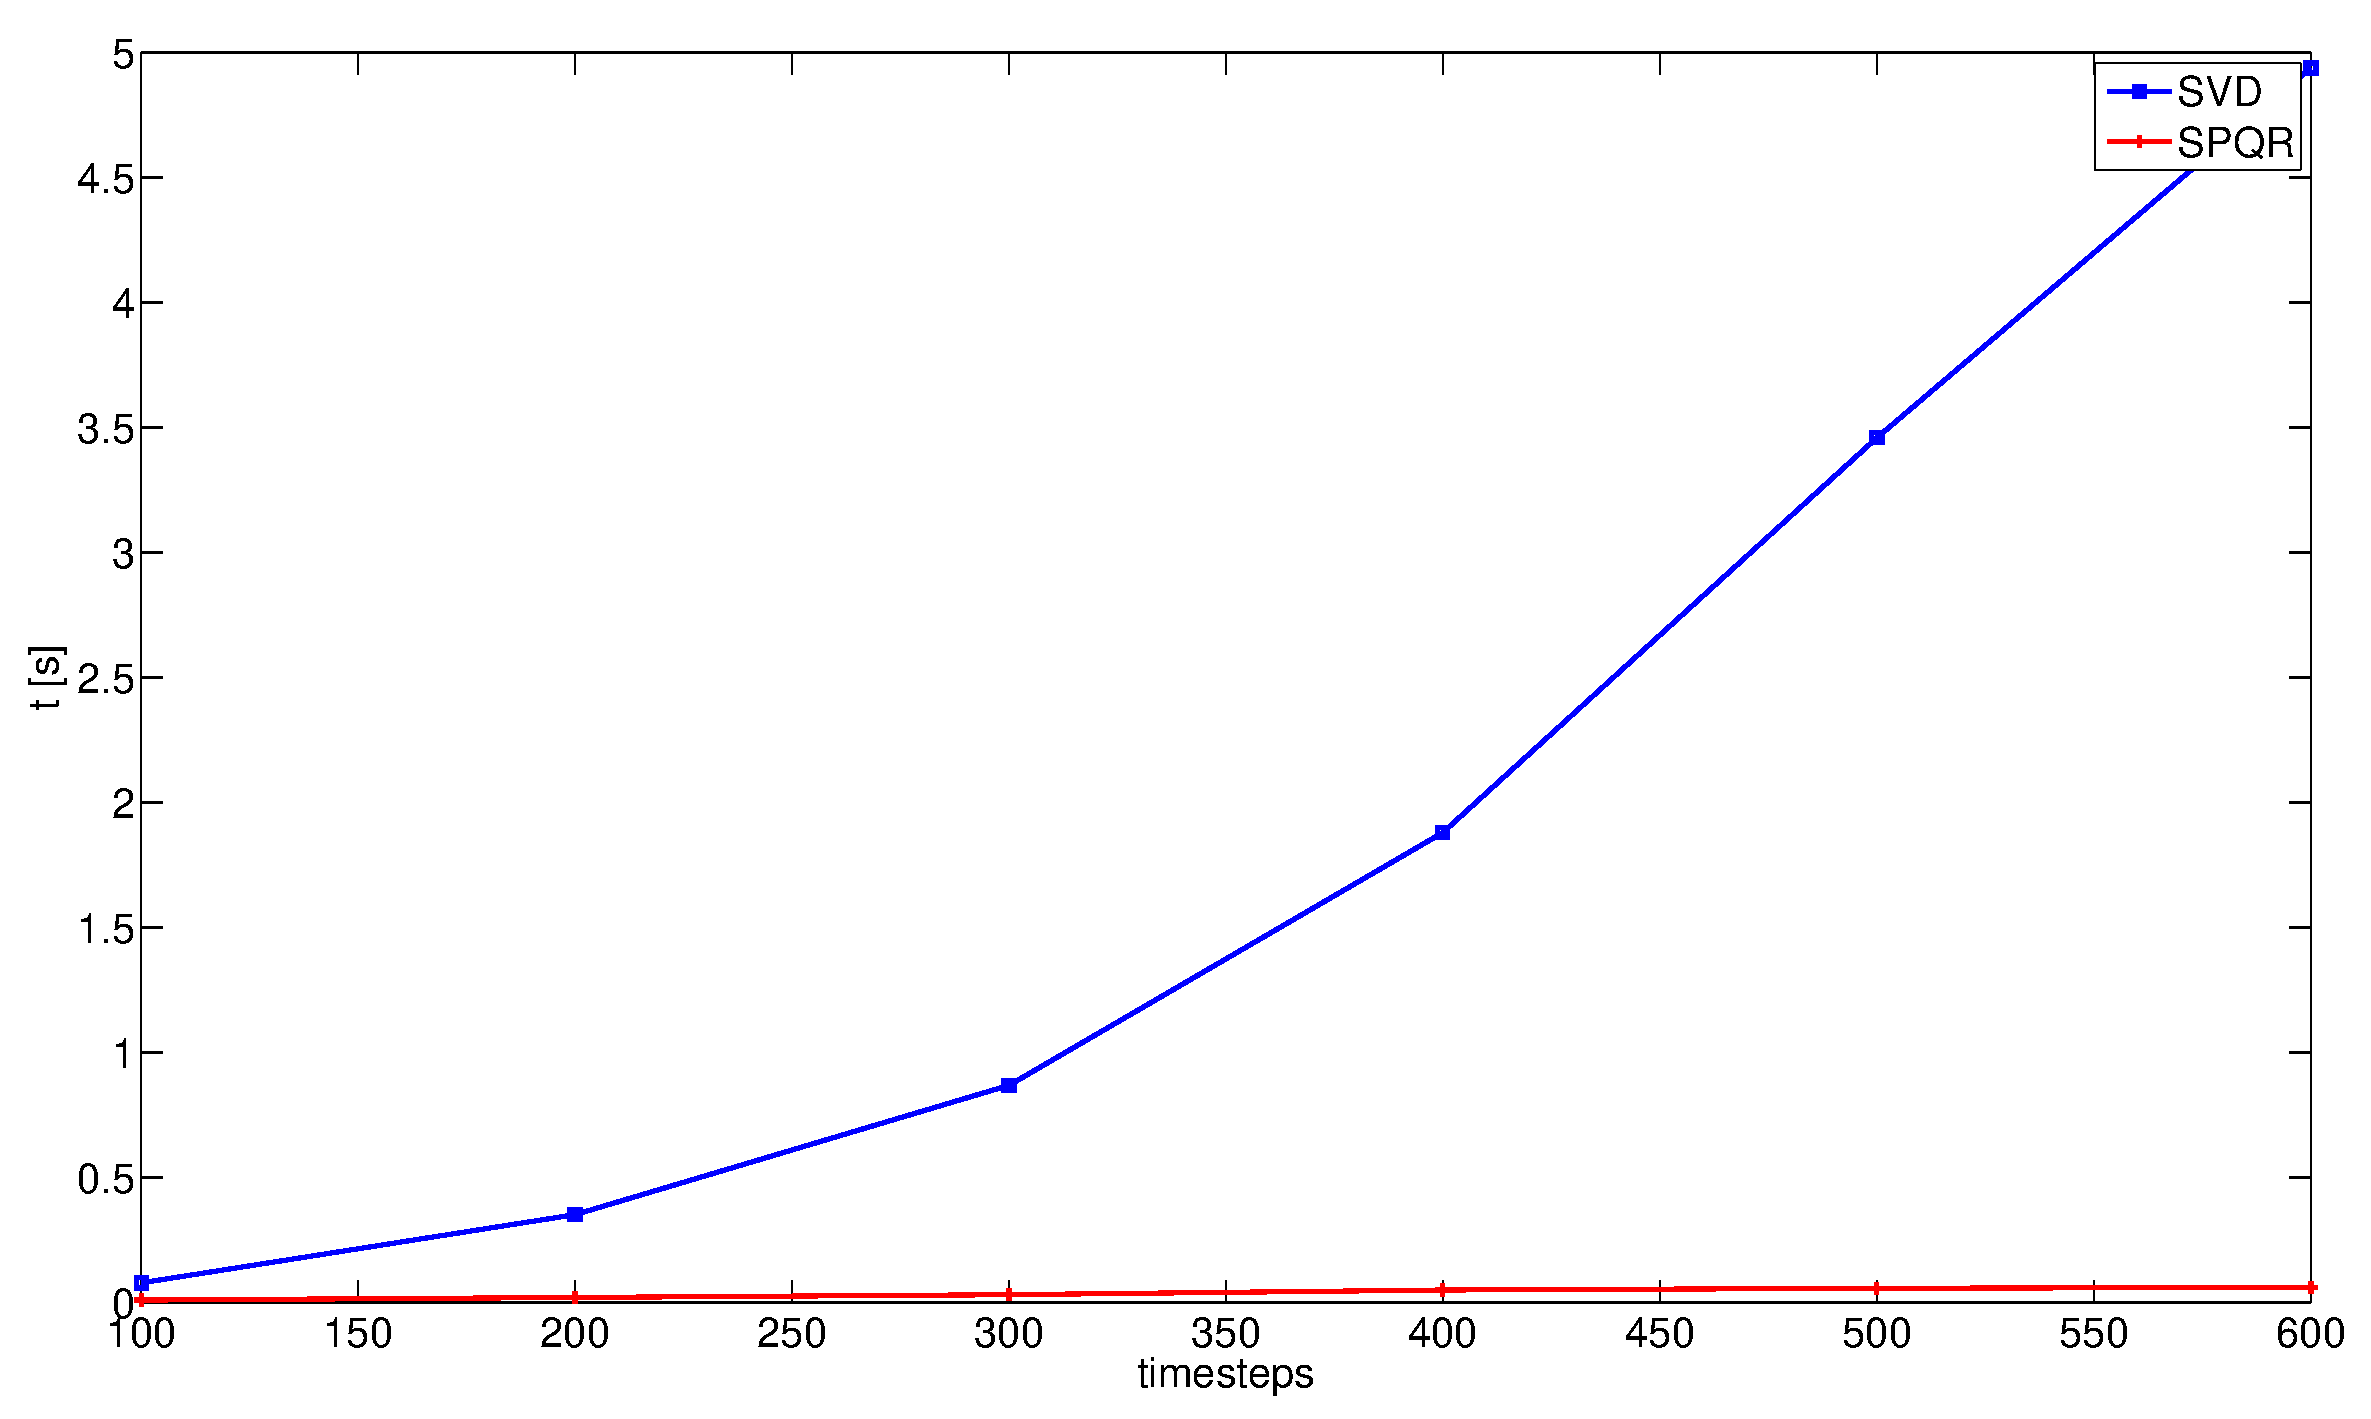
\includegraphics[width=\columnwidth]{fig/straight-path-time.eps}
\caption{Mean computation time over 100 repetitions for one step of
  optimization using SVD (polynomial time) and sparse QR (linear time)
  decomposition.}
\label{fig:straight-path-time}
\end{figure}

To conclude this section on simulated data, we will analyze the performance of
different algorithms, namely an Extended Kalman Filter (EKF) similar
to~\cite{martinelli06automatic}, a standard batch nonlinear least squares
method without regularization~\cite{kuemmerle11simultaneous}, and our TQR-MI
approach, on a sine wave path with varying amplitude such that the offset
parameters range from unobservable (straight path or zero amplitude) to
fully observable (higher amplitude). To get significant statistical results, we
have repeated the experiment $100$ times with the same initial conditions
($\delta_x^{(0)}=0.22$ [m], $\delta_y^{(0)}=0.12$ [m], $\psi^{(0)}=0.8$ [rad])
and amplitudes from $0$ [m] to $3$ [m] with steps of $0.5$ [m].

\subsection{Real-world Data}

In order to validate our method on real-world data, we have used the ``Lost in
the Woods Dataset'' provided with the courtesy of Tim
Barfoot~\cite{tong12gaussian}. This dataset contains approximately $20$ minutes
of a robot driving amongst a forest of tubes which serve as landmarks. The
ground truth comes from a motion capture system that tracks robot motion and
tube locations. For the calibration parameters, we have only access to
$\delta_x=0.219$ [m] that was roughly measured with a tape. We assume the others
are implicitly set to $0$ ($\delta_y=0$ [m] and $\psi=0$ [rad]).
Fig.~\ref{fig:dataset2-path-result} displays the qualitative result of our
algorithm. Using only $10\%$ of the measurements, we could recover accurate
landmark positions, robot poses, and calibration parameters. For visualization,
estimated landmarks and poses have
been aligned to the ground truth using the algorithm
from~\cite{fiore01efficient}.

\begin{figure}[t]
\centering
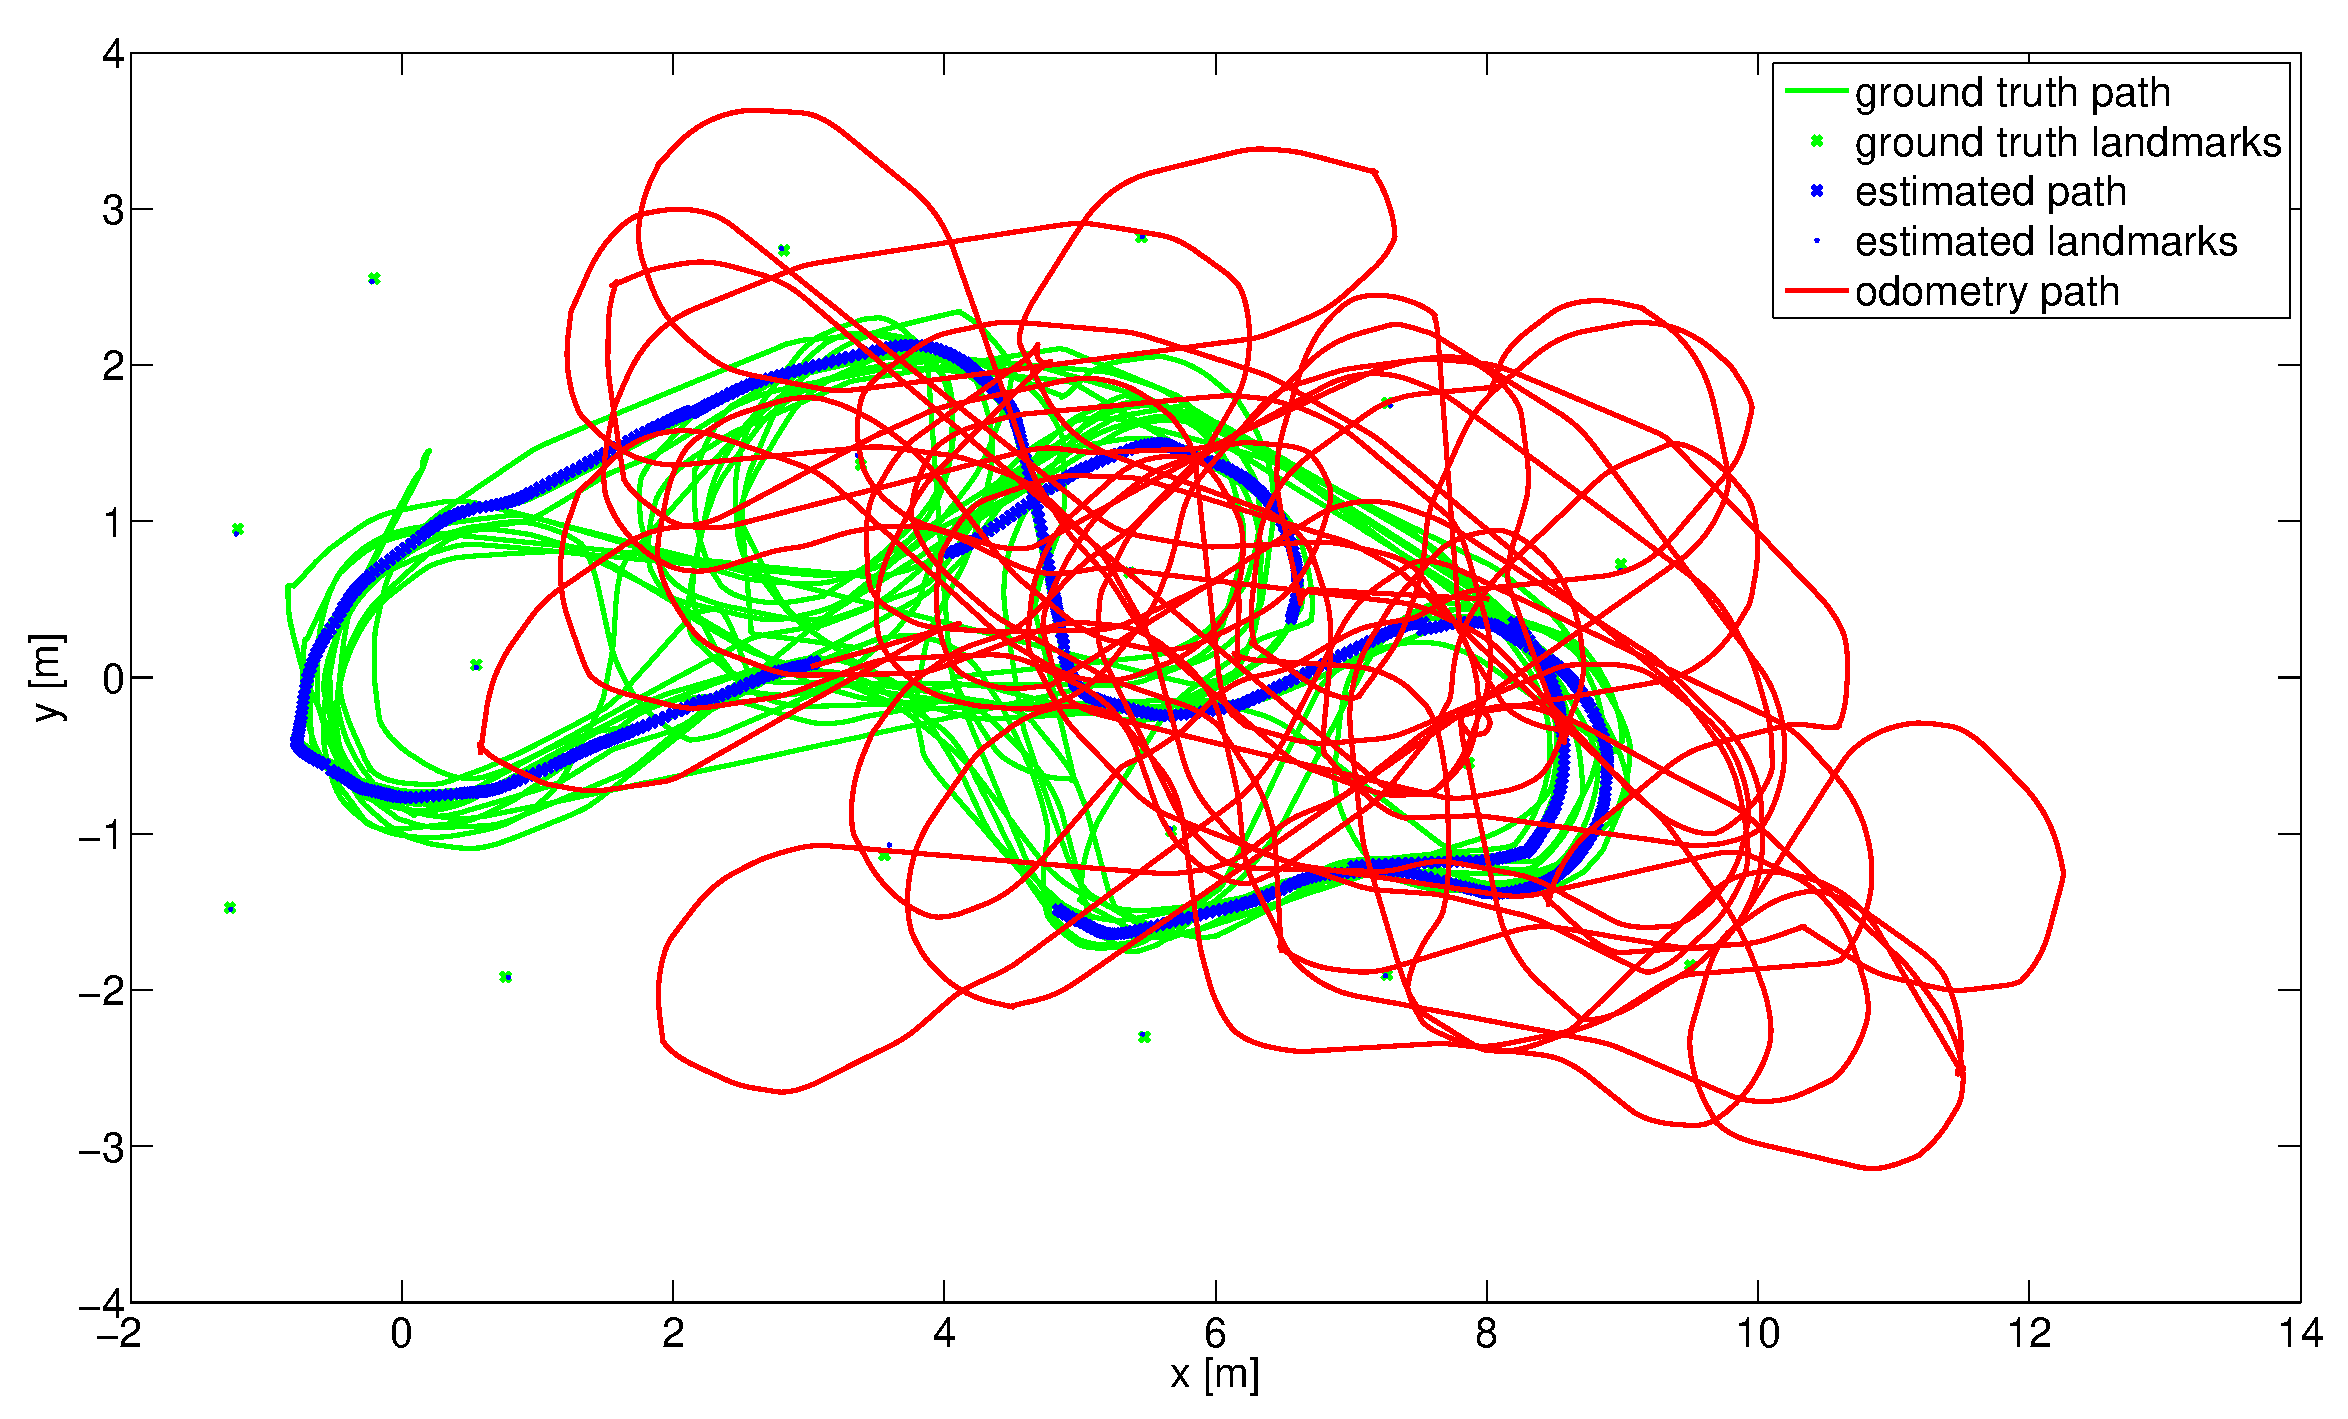
\includegraphics[width=\columnwidth]{fig/dataset2-path-result.eps}
\caption{Application of our algorithm on the ``Lost in the Woods dataset''
  (best viewed in color). The
  green line represents the ground truth path, the red line the integrated
  odometry path, the green crosses the ground truth landmark positions, the blue
  points the estimated landmark positions, and the blue crosses the estimated
  robot poses. Our MI selection scheme picks only $10\%$ of the measurements
  for the optimization.}
\label{fig:dataset2-path-result}
\end{figure}

Since the ground truth calibration parameters are inaccurate,
Tab.~\ref{tab:dataset2-comp} compares our method against a standard
least squares (LS) estimator that exploits all the measurements. Our TQR-MI
algorithm performs the optimization with $K=1209$ out of $12609$ timesteps.
Although the calibration parameters are the same magnitude, the higher variances
stem from the fewer number of considered measurements.

\begin{table}[!t]
\renewcommand{\arraystretch}{1.3}
\caption{Comparison of a standard least squares estimator and our
  method on the ``Lost in the Woods dataset''.}
\label{tab:dataset2-comp}
\centering
\begin{tabular}{c||c||c}
\hline
& \bfseries LS & \bfseries TQR-MI\\
\hline\hline
$\hat{\delta}_x$ [m] & $0.2363$ & $0.2344$\\
\hline
$\hat{\delta}_y$ [m]& $0.0034$ & $0.0087$\\
\hline
$\hat{\psi}$ [rad] & $0.0810$ & $0.0754$\\
\hline
$\hat{\Sigma}_{\delta_x}$ [$\text{m}^2$] & $0.0892\times 10^{-5}$ &
  $0.1903\times 10^{-4}$\\
\hline
$\hat{\Sigma}_{\delta_y}$ [$\text{m}^2$] & $0.39\times 10^{-5}$ &
  $0.7243\times 10^{-4}$\\
\hline
$\hat{\Sigma}_{\psi}$ [$\text{rad}^2$] & $0.0254\times 10^{-5}$ &
  $0.0582\times 10^{-4}$\\
\hline
$K$ & $12609$ & $1209$\\
\hline
\end{tabular}
\end{table}
